
\section{Experiments}

\subsection{Synthetic Dataset}


To illustrate our theoretical claims, we start by testing our learning algorithm on the following synthetic two-dimensional problem. Let us consider the distribution $\PP$ defined as  $\PP\left(Y =\pm 1\right)=1/2$, $\PP\left(X\mid Y=-1\right) = \mathcal{N}(0,I_2)$ and $\PP\left(X \mid Y=1\right) = \frac12\left[\mathcal{N}((-3,0),I_2)+\mathcal{N}((3,0),I_2) \right]$.
% \begin{align*}
%   \left\{
%     \begin{array}{ll}
%   \\
%         \PP\left(X\mid Y=-1\right) = \mathcal{N}(0,I_2) \\
%         \PP\left(X \mid Y=1\right) = \frac12\left[\mathcal{N}((-3,0),I_2)+\mathcal{N}((3,0),I_2) \right].
%     \end{array}
% \right. 
% \end{align*}
We sample $1000$ training points from this distribution and randomly generate $10$ linear classifiers that achieves a standard training risk lower than $0.4$. To simulate an adversary with budget $\varepsilon$ in $\ell_2$ norm, we proceed as follows. For every sample $(x,y)\sim \PP$ we generate $1000$ points uniformly at random in the ball of radius $\varepsilon$ and select the one maximizing the risk for the $0/1$ loss. Figure~\ref{fig:toy_example} (left) illustrates the type of mixtures we obtain after convergence of our algorithms. Note that in this toy problem, we are likely to find the optimal adversary with this sampling strategy if we sample enough attack points. 
% \begin{figure}[ht]
%     \centering
%     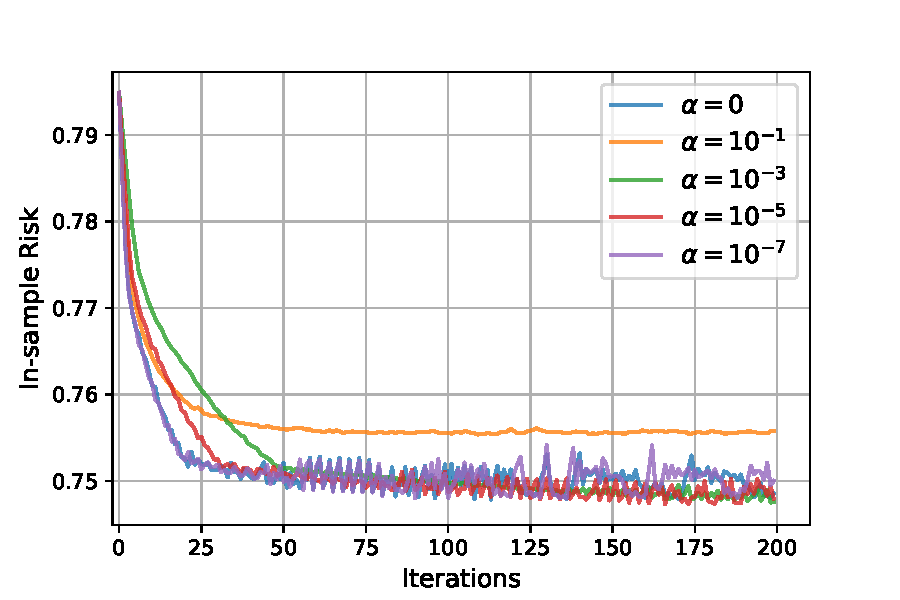
\includegraphics[width=0.46\textwidth]{Images/convergence_toy.pdf}
%     \caption{Caption}
%     \label{fig:toy_example_cvgence}
% \end{figure}
\begin{figure*}[!ht]
\begin{center}

\textbf{Adversarial Training, CIFAR-10 dataset results}
 \begin{scriptsize}
\begin{tabular}{c|c|ccc} 
\textbf{ Models} & \textbf{Acc. }&\textbf{$\textrm{APGD}_\textrm{CE}$}& \textbf{$\textrm{APGD}_\textrm{DLR}$} & \textbf{Rob. Acc.} \\ \hline
 1 & $81.9\%$ &	$47.6\%$ & $47.7\%$ & $45.6\%$ \\ 
 2 & $81.9\%$ & $49.0\%$ & ${49.6\%}$ & ${47.0\%}$\\ 
  3 & ${81.7\%}$& ${49.0\%}$ & $49.3\%$ & ${46.9\%}$\\
    4 & $\bm{82.6\%}$& $\bm{49.7\%}$ & $\bm{49.8}\%$ & $\bm{47.2\%}$\\

\end{tabular}
\end{scriptsize}\\
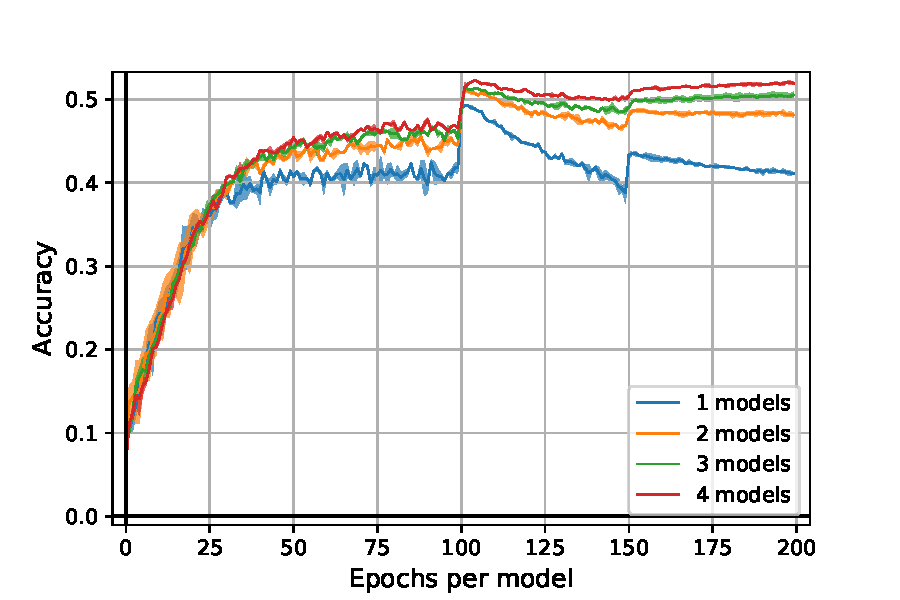
\includegraphics[width=0.35\textwidth]{Images/robust_acc_finalrun_ResNet18_1024_200_0.001.pdf}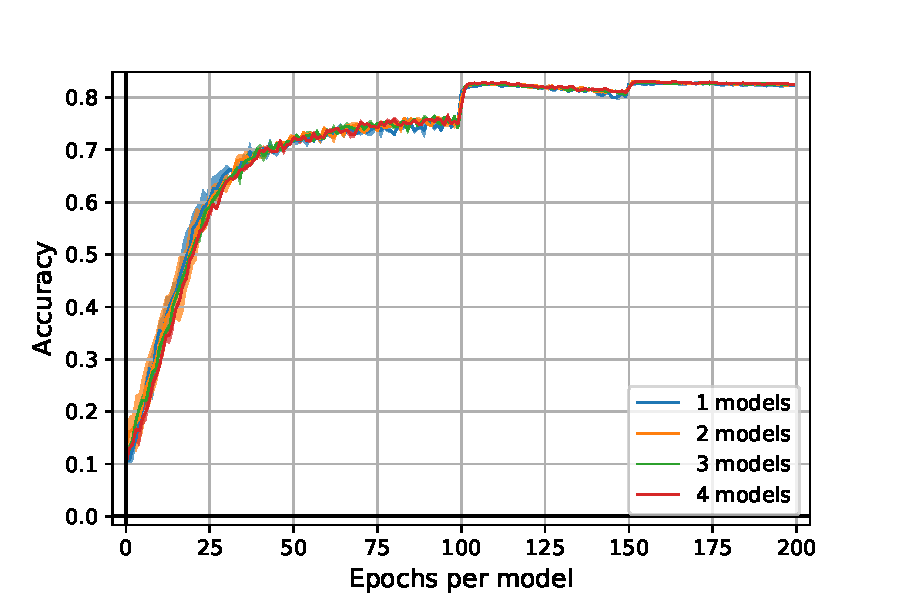
\includegraphics[width=0.35\textwidth]{Images/standard_acc_finalrun_ResNet18_1024_200_0.001.pdf} 
  

\textbf{TRADES, CIFAR-10 dataset results}

 \begin{scriptsize}
\begin{tabular}{c|c|ccc} 
\textbf{ Models} & \textbf{Acc. }&\textbf{$\textrm{APGD}_\textrm{CE}$}& \textbf{$\textrm{APGD}_\textrm{DLR}$} & \textbf{Rob. Acc.} \\ \hline
 1 &  $79.6\%$ &$50.9\%$& $48.9\%$ &$48.3\%$ \\ 
 2 & $80.3\%$& $52.3\%$ &$51.2\%$ &$50.2\%$\\ 
  3 & $80.7\%$& $52.8\%$ &$51.7\%$ &$50.7\%$\\
    4 & \bm{$80.9\%$} & \bm{$53.0\%$}& \bm{$51.8\%$}& \bm{$50.8\%$}\\

\end{tabular}
\end{scriptsize}

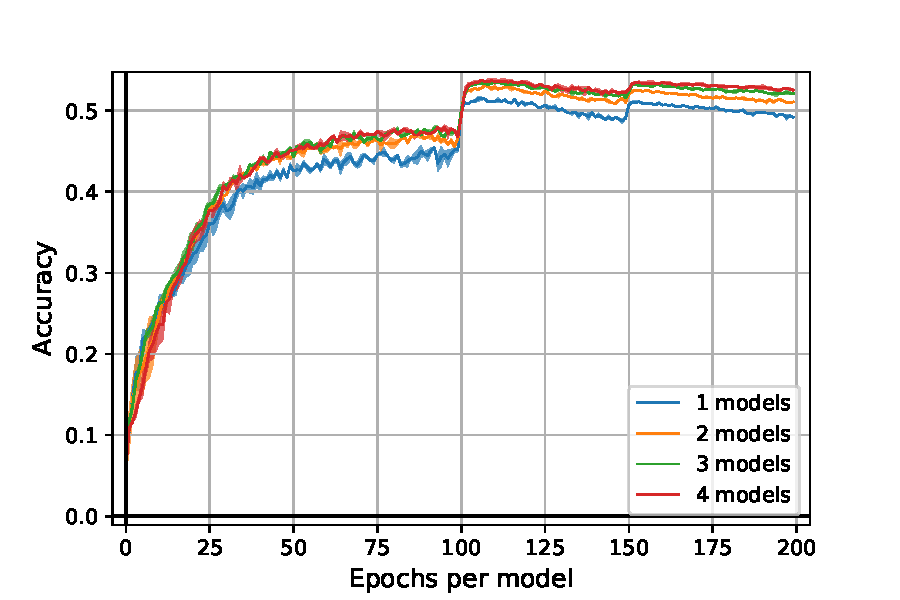
\includegraphics[width=0.35\textwidth]{Images/robust_acc_CIFAR10_final_cam_ready_bisss_ResNet18_1024_200_0.001.pdf}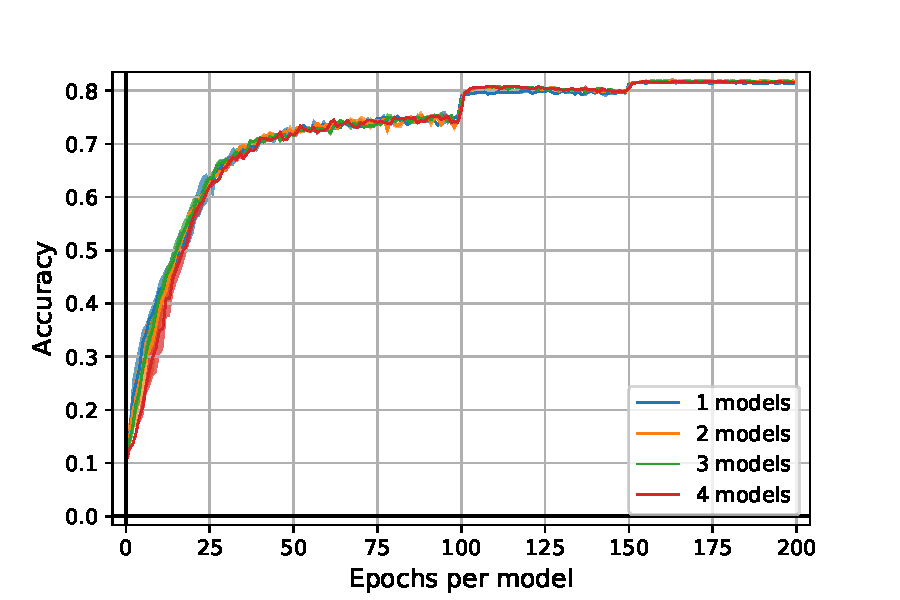
\includegraphics[width=0.35\textwidth]{Images/standard_acc_CIFAR10_final_cam_ready_bisss_ResNet18_1024_200_0.001.pdf} 
  

\textbf{Adversarial Training, CIFAR-100 dataset results}
 \begin{scriptsize}
\begin{tabular}{c|c|ccc} 
\textbf{ Models} & \textbf{Acc. }&\textbf{$\textrm{APGD}_\textrm{CE}$}& \textbf{$\textrm{APGD}_\textrm{DLR}$} & \textbf{Rob. Acc.} \\ \hline
 1 & $55.2\%$& $24.1\%$& $23.8\%$ & $22.5\%$\\ 
 2 & $55.2\%$ & $25.3\%$ &$26.1\%$ &$23.6\%$\\ 
  3 & \bm{$55.4\%$} & $25.7\%$ &$26.8\%$ &$24.2\%$\\
    4 & $55.3\%$ & \bm{$26.0\%$} & \bm{$27.5\%$}& \bm{$24.5\%$}\\

\end{tabular}
\end{scriptsize}
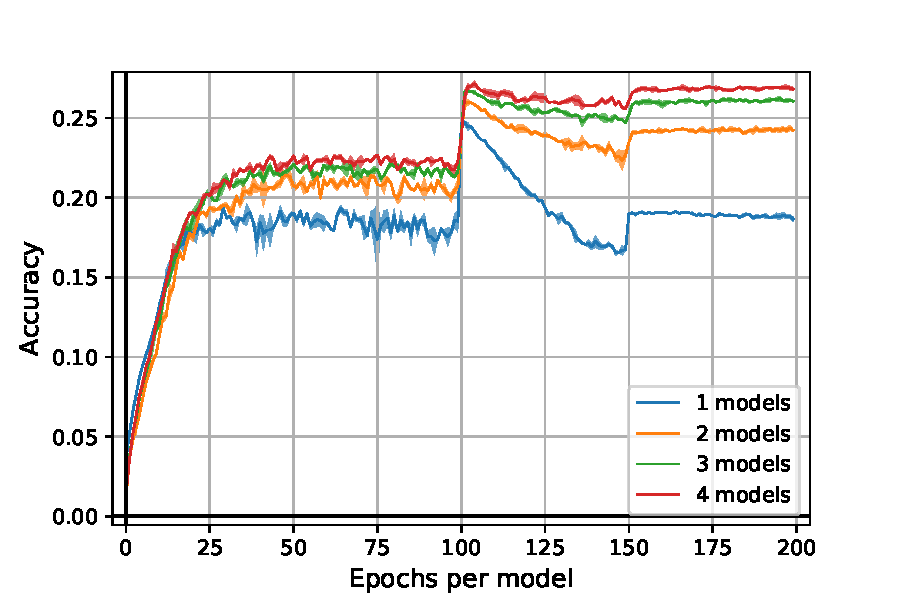
\includegraphics[width=0.35\textwidth]{Images/robust_acc_CIFAR100_finalrun_ResNet18_1024_200_0.001.pdf}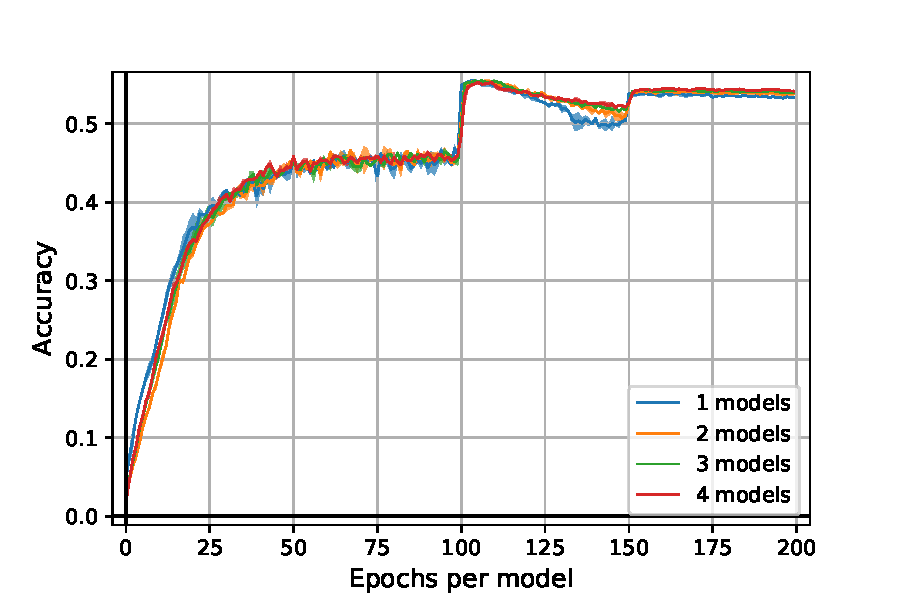
\includegraphics[width=0.35\textwidth]{Images/standard_acc_CIFAR100_finalrun_ResNet18_1024_200_0.001.pdf} 


 \caption{Upper plots: Adversarial Training, CIFAR-10 dataset results. Middle plots:  TRADES, CIFAR-10 dataset results. Bottom plots: CIFAR-100 dataset results. {On left}: Comparison of our algorithm with a standard adversarial training (one model). We reported the results for the model with the best robust accuracy obtained over two independent runs because adversarial training might be unstable. Standard and Robust accuracy (respectively in the middle and on right) on CIFAR-10 test images in function of the number of epochs per classifier with $1$ to $3$ ResNet18 models. The performed attack is PGD with $20$ iterations and $\varepsilon=8/255$.}
\label{fig:results_cifar}

\end{center}
\end{figure*}

To evaluate the convergence of our algorithms, we compute the adversarial risk of our mixture for each iteration of both the oracle and regularized algorithms. Figure~\ref{fig:toy_example} illustrates the convergence of the algorithms w.r.t the regularization parameter. We observe that the risk for both algorithms converge. Moreover, they converge towards the oracle minimizer when the regularization parameter $\alpha$ goes to $0$.

Finally, to demonstrate the improvement randomized techniques offer against deterministic defenses, we plot in Figure~\ref{fig:toy_example} (right) the minimum adversarial risk for both randomized and deterministic classifiers w.r.t. $\varepsilon$. The adversarial risk is strictly better for randomized classifier whenever the adversarial budget $\varepsilon$ is bigger than $2$. This illustration corroborates our analysis of Theorem~\ref{thm:duality-rand}, and motivates an in-depth study of a more challenging framework, namely image classification with neural networks.

% \begin{figure}[ht]
%     \centering
%     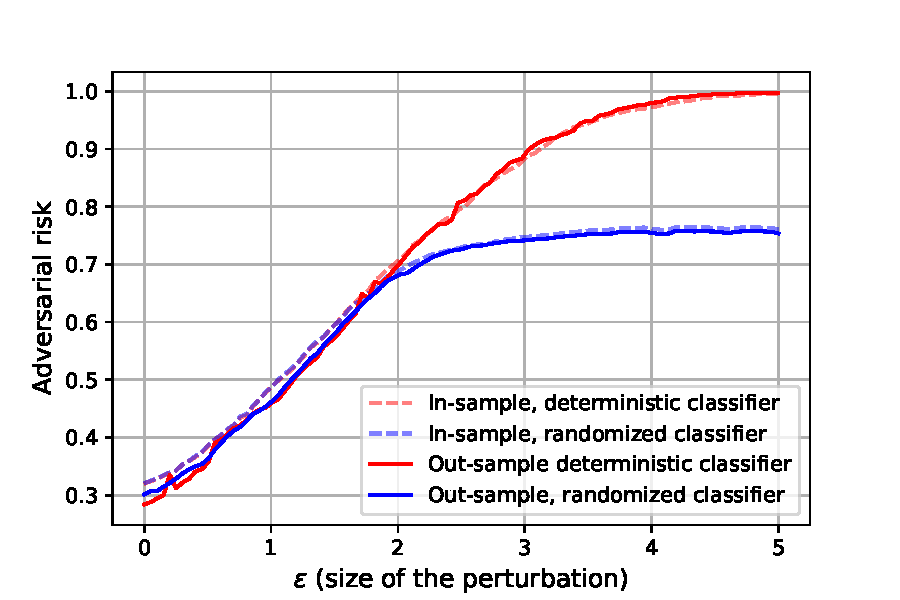
\includegraphics[width=0.46\textwidth]{Images/risk_toy.pdf}
%     \caption{Caption}
%     \label{fig:toy_example_risk}
% \end{figure}

\subsection{CIFAR Datasets}

% \begin{figure*}[!ht]
% \begin{center}

% \vskip 0.15in
%  \begin{minipage}[ht!]{0.39\textwidth}
%  \begin{scriptsize}
% \begin{tabular}{c|c|ccc} 
% \textbf{ Models} & \textbf{Acc. }&\textbf{$\textrm{APGD}_\textrm{CE}$}& \textbf{$\textrm{APGD}_\textrm{DLR}$} & \textbf{Rob. Acc.} \\ \hline
%  1 & $81.9\%$ &	$47.6\%$ & $47.7\%$ & $45.6\%$ \\ 
%  2 & $81.9\%$ & $49.0\%$ & ${49.6\%}$ & ${47.0\%}$\\ 
%   3 & ${81.7\%}$& ${49.0\%}$ & $49.3\%$ & ${46.9\%}$\\
%     4 & $\bm{82.6\%}$& $\bm{49.7\%}$ & $\bm{49.8}\%$ & $\bm{47.2\%}$\\

% \end{tabular}
% \end{scriptsize}
%   \end{minipage}\begin{minipage}[!ht]{0.61\textwidth}
% 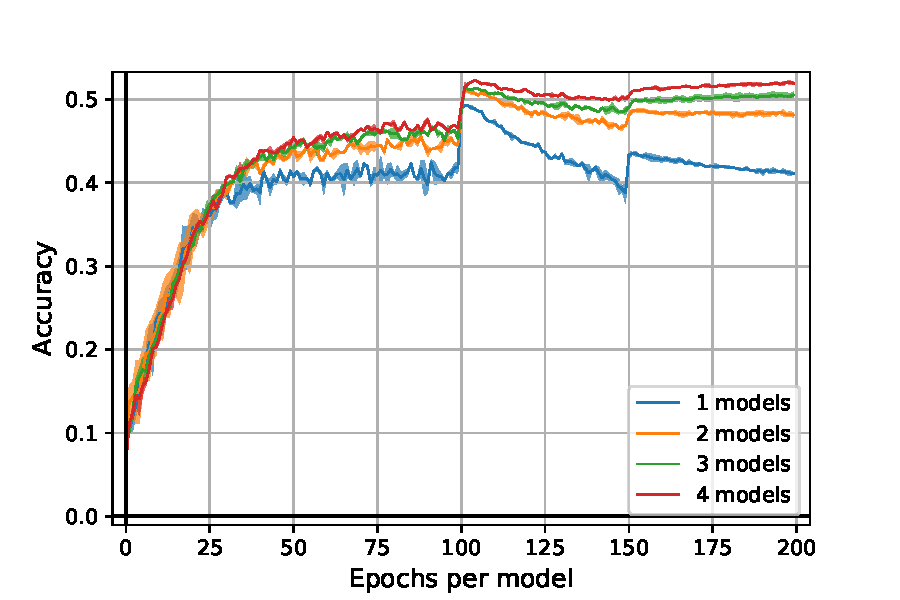
\includegraphics[width=0.49\textwidth]{Images/robust_acc_finalrun_ResNet18_1024_200_0.001.pdf}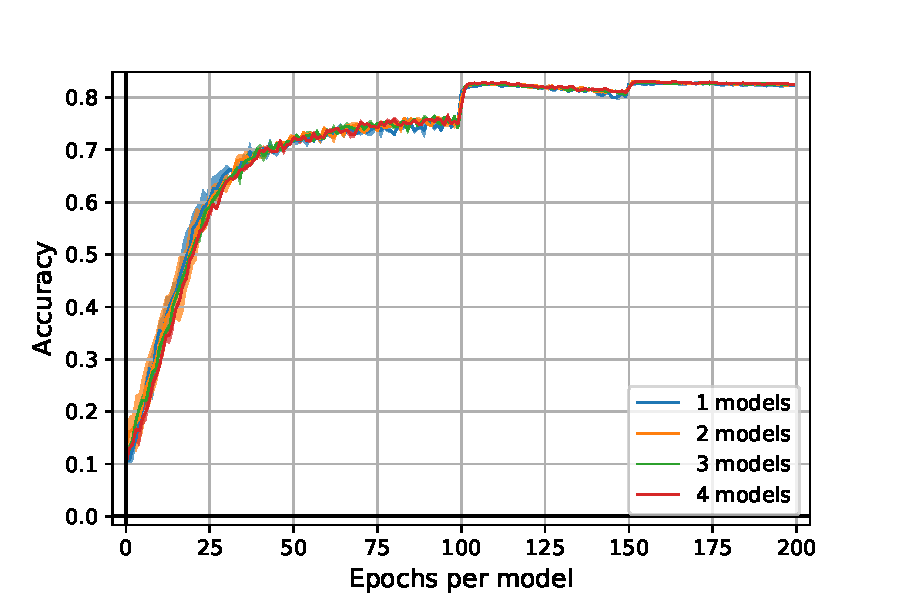
\includegraphics[width=0.49\textwidth]{Images/standard_acc_finalrun_ResNet18_1024_200_0.001.pdf} 
%   \end{minipage}
  
% Adversarial Training, CIFAR-10 dataset results

% \vskip 0.15in
%  \begin{minipage}[ht!]{0.39\textwidth}
%  \begin{scriptsize}
% \begin{tabular}{c|c|ccc} 
% \textbf{ Models} & \textbf{Acc. }&\textbf{$\textrm{APGD}_\textrm{CE}$}& \textbf{$\textrm{APGD}_\textrm{DLR}$} & \textbf{Rob. Acc.} \\ \hline
%  1 &  $79.6\%$ &$50.9\%$& $48.9\%$ &$48.3\%$ \\ 
%  2 & $80.3\%$& $52.3\%$ &$51.2\%$ &$50.2\%$\\ 
%   3 & $80.7\%$& $52.8\%$ &$51.7\%$ &$50.7\%$\\
%     4 & \bm{$80.9\%$} & \bm{$53.0\%$}& \bm{$51.8\%$}& \bm{$50.8\%$}\\

% \end{tabular}
% \end{scriptsize}
%   \end{minipage}\begin{minipage}[!ht]{0.61\textwidth}
% 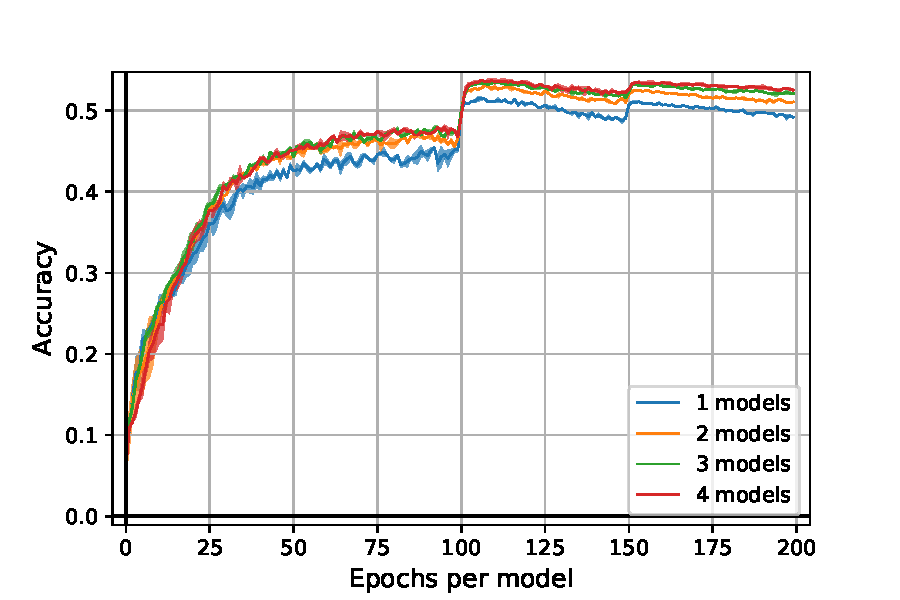
\includegraphics[width=0.49\textwidth]{Images/robust_acc_CIFAR10_final_cam_ready_bisss_ResNet18_1024_200_0.001.pdf}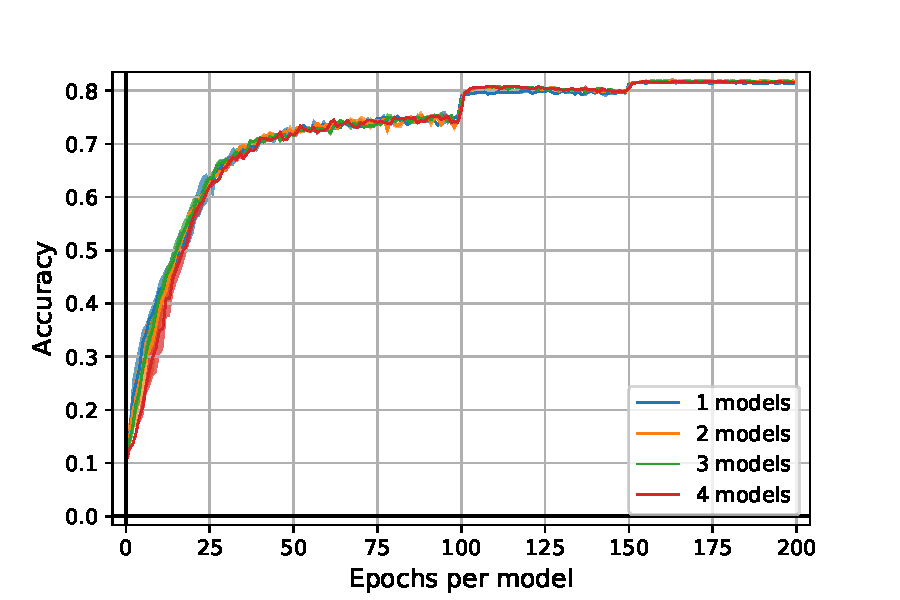
\includegraphics[width=0.49\textwidth]{Images/standard_acc_CIFAR10_final_cam_ready_bisss_ResNet18_1024_200_0.001.pdf} 
%   \end{minipage}
  
% TRADES, CIFAR-10 dataset results
% \vskip 0.15in
%  \begin{minipage}[ht!]{0.39\textwidth}
%  \begin{scriptsize}
% \begin{tabular}{c|c|ccc} 
% \textbf{ Models} & \textbf{Acc. }&\textbf{$\textrm{APGD}_\textrm{CE}$}& \textbf{$\textrm{APGD}_\textrm{DLR}$} & \textbf{Rob. Acc.} \\ \hline
%  1 & $55.2\%$& $24.1\%$& $23.8\%$ & $22.5\%$\\ 
%  2 & $55.2\%$ & $25.3\%$ &$26.1\%$ &$23.6\%$\\ 
%   3 & \bm{$55.4\%$} & $25.7\%$ &$26.8\%$ &$24.2\%$\\
%     4 & $55.3\%$ & \bm{$26.0\%$} & \bm{$27.5\%$}& \bm{$24.5\%$}\\

% \end{tabular}
% \end{scriptsize}
%   \end{minipage}\begin{minipage}[!ht]{0.61\textwidth}
% 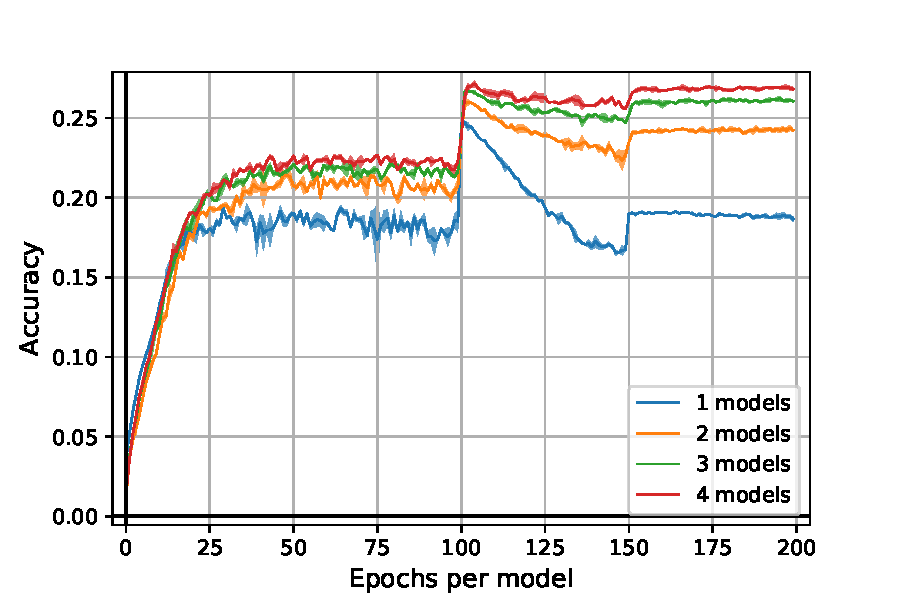
\includegraphics[width=0.49\textwidth]{Images/robust_acc_CIFAR100_finalrun_ResNet18_1024_200_0.001.pdf}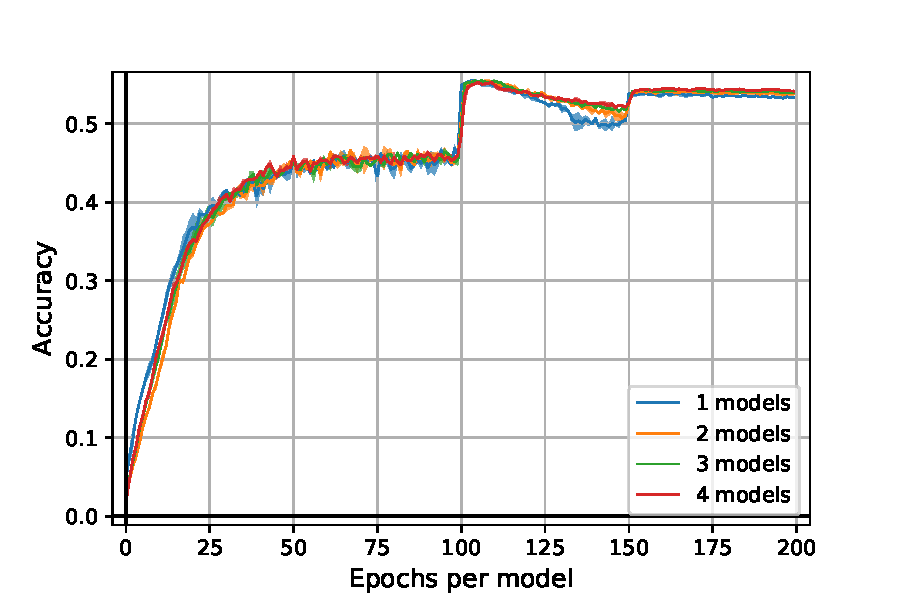
\includegraphics[width=0.49\textwidth]{Images/standard_acc_CIFAR100_finalrun_ResNet18_1024_200_0.001.pdf} 
%   \end{minipage}
%   Adversarial Training, CIFAR-100 dataset results

%  \caption{Upper plots: Adversarial Training, CIFAR-10 dataset results. Middle plots:  TRADES, CIFAR-10 dataset results. Bottom plots: CIFAR-100 dataset results. {On left}: Comparison of our algorithm with a standard adversarial training (one model). We reported the results for the model with the best robust accuracy obtained over two independent runs because adversarial training might be unstable. Standard and Robust accuracy (respectively in the middle and on right) on CIFAR-10 test images in function of the number of epochs per classifier with $1$ to $3$ ResNet18 models. The performed attack is PGD with $20$ iterations and $\varepsilon=8/255$.}
% \label{fig:results_cifar}

% \end{center}
% \end{figure*}

% Adversarial examples are known to be easily transferrable from one model to another~\cite{tramer2017space}. To counter this and support our theoretical claims, we propose an heuristic algorithm (see Algorithm~\ref{algo:heuristic}) to train a robust mixture of $L$ classifiers. We alternatively train these classifiers with adversarial examples against the current mixture and update the probabilities of the mixture according to the algorithms we proposed in Section~\ref{sec:proposed-algo}. More details on the heuristic algorithm are available in Appendix~\ref{sec:additional-xp}. 
% \begin{algorithm}[h!]
% \small
% \SetAlgoLined
% $L$: number of models, $T$: number of iterations,\\
% $T_\theta$: number of updates for the models $\bm{\theta}$,\\
% $T_\lambda$: number of updates for the mixture $\bm{\lambda}$,\\ $\bm{\lambda}_0=(\lambda_0^1,\dots\lambda_0^L),~\bm{\theta}_0=(\theta_0^1,\dots\theta_0^L)$\\
%  \For{$t=1,\dots,T$}{
%  Let $B_t$ be a batch of data.\\
% \eIf{$t \mod (T_\theta L+1)\neq 0$}{
% $k$ sampled uniformly in $\{1,\dots,L\}$\\
% $\Tilde{B}_t\leftarrow$ Attack of images in $B_t$ for the  model $(\bm{\lambda}_t,\bm{\theta}_t)$\\
% $\theta^t_k\leftarrow$ Update $\theta^{t-1}_k$ with $\Tilde{B}_t$ for fixed $\bm{\lambda}_t$ with a SGD step}{
% $\bm{\lambda}_t\leftarrow$Update $\bm{\lambda}_{t-1}$ on $B_t$ for fixed $\bm{\theta}_t$
% with oracle or regularized algorithm with $T_\lambda$ iterations.
% }
%   }
%  \caption{Adversarial Training for Mixtures}
 
%  \label{algo:heuristic}
% \end{algorithm}

\paragraph{Experimental Setup.} We now implement our heuristic algorithm (Alg.~\ref{algo:heuristic}) on CIFAR-10 and CIFAR-100 datasets for both Adversarial Traning~\citep{madry2018towards} and TRADES~\citep{zhang2019theoretically} loss. To evaluate the performance of Algorithm~\ref{algo:heuristic}, we trained from $1$ to $4$ ResNet18~\citep{he2016deep} models on $200$ epochs per model\footnote{$L\times200$ epochs in total, where $L$ is the number of models.}. We study the robustness with regards to $\ell_\infty$ norm and fixed adversarial budget $\varepsilon=8/255$. The attack we used in the inner maximization of the training is an adaptative version of PGD for mixtures of classifiers with $10$ steps. Note that for one single model, Algorithm~\ref{algo:heuristic} exactly corresponds to adversarial training~\citep{madry2018towards} or TRADES. For each of our setups, we made two independent runs and select the  best one. The training time of our algorithm is around four times longer than a standard Adversarial Training (with PGD 10 iter.) with two models, eight times with three models and twelve times with four models. We trained our models with a batch of size  $1024$ on $8$ Nvidia V100 GPUs. 

\paragraph{Evaluation Protocol.} At each epoch, we evaluate the current mixture on test data against PGD attack  with $20$ iterations. To select our model and avoid overfitting~\citep{rice2020overfitting}, we kept the most robust against this PGD attack.
To make a final evaluation of our mixture of models, we used an adapted version of {AutoPGD} (APGD) untargeted attacks~\citep{croce2020reliable} for randomized classifiers with both Cross-Entropy (CE) and Difference of Logits Ratio (DLR) loss. For both attacks, we made $100$ iterations and $5$ restarts.

\paragraph{Optimizer.} For each of our models, The optimizer we used in all our implementations is SGD with learning rate set to $0.4$ at epoch $0$ and is divided by $10$ at half training then by $10$ at the three quarters of training. The momentum is set to $0.9$ and the weight decay to $5\times10^{-4}$. The batch size is set to $1024$. 
\paragraph{Adaptation of Attacks.} Since our classifier is randomized, we need to adapt the attack accordingly. To do so we used the expected loss:
\begin{align*}
\Tilde{\loss}\left((\bm{\lambda},\bm{\theta}),(x,y)\right) = \sum_{k=1}^l \lambda_k \loss(\theta_k,(x,y))
\end{align*}
to compute the gradient in the attacks, regardless the loss (DLR or CE). For the inner maximization at training time, we used a PGD attack on the cross-entropy loss with $\varepsilon=0.03$. 
\paragraph{Regularization in Practice.} The entropic regularization in higher dimensional setting need to be adapted to be more likely to find adversaries. To do so, we computed PGD attacks with only $3$ iterations with $5$ different restarts instead of sampling uniformly $5$ points  in the $\ell_\infty$-ball. In our experiments in the main paper, we use a regularization parameter $\alpha=0.001$. The learning rate for the minimization on $\bm{\lambda}$ is always fixed to $0.001$. 
\paragraph{Alternate Minimization Parameters.} Algorithm~\ref{algo:heuristic} implies an alternate minimization algorithm. We set the number of updates of $\bm{\theta}$ to $T_\theta = 50$ and, the update of $\bm{\lambda}$ to $T_\lambda = 25$. 

\subsection{Effect of the Regularization}
In this subsection, we experimentally investigate the effect of the regularization. In Figure~\ref{fig:xp-regularization}, we notice that the regularization has the effect of stabilizing, reducing the variance and improving the level of the robust accuracy for adversarial training of mixtures (Algorithm~\ref{algo:heuristic}). The standard accuracy curves are very similar in both cases.





\paragraph{Results.} The results are presented in Figure~\ref{fig:results_cifar}. We remark our algorithm outperforms the standard adversarial training procedure in all the cases by more $1\%$ on CIFAR-10 and CIFAR-100, without additional loss of standard accuracy as it is shown in the left figures. On TRADES, the gain is even more important by more than $2\%$ in robust accuracy. Moreover, it seems that our algorithm, by adding more and more models, reduces the overfitting of adversarial training. It also appears that robustness increases as the number of models increases. So far, experiments are computationally very costly, and it is difficult to draw precise conclusions. Further, hyperparameter tuning ~\citep{gowal2020uncovering} such as architecture, unlabeled data~\citep{carmon2019unlabeled} or activation function may still improve the results.





% \begin{figure*}[!ht]
% \begin{center}


% \label{table:results}
% \vskip 0.15in
%  \begin{minipage}[!ht]{0.39\textwidth}
%  \begin{scriptsize}
% \begin{tabular}{c|c|ccc} 
% \textbf{ Models} & \textbf{Acc. }&\textbf{$\textrm{APGD}_\textrm{CE}$}& \textbf{$\textrm{APGD}_\textrm{DLR}$} & \textbf{Rob. Acc.} \\ \hline
%  1 & $81.9\%$ &	$47.6\%$ & $47.7\%$ & $45.6\%$ \\ 
%  2 & $81.9\%$ & $49.0\%$ & ${49.6\%}$ & ${47.0\%}$\\ 
%   3 & ${81.7\%}$& ${49.0\%}$ & $49.3\%$ & ${46.9\%}$\\
%     4 & $\bm{82.6\%}$& $\bm{49.7\%}$ & $\bm{49.8}\%$ & $\bm{47.2\%}$\\

% \end{tabular}
% \end{scriptsize}
%   \end{minipage}\begin{minipage}[!ht]{0.61\textwidth}
% 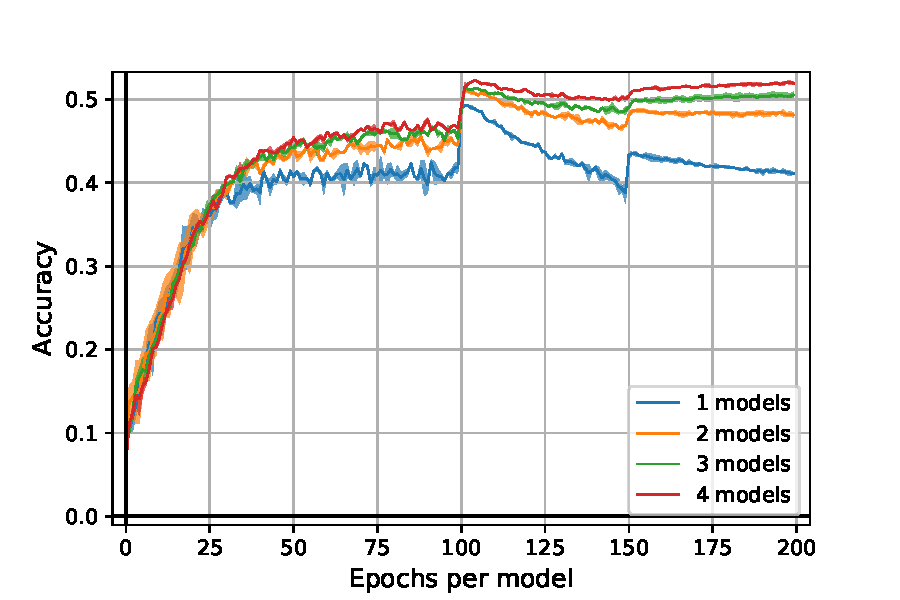
\includegraphics[width=0.49\textwidth]{Images/robust_acc_finalrun_ResNet18_1024_200_0.001.pdf}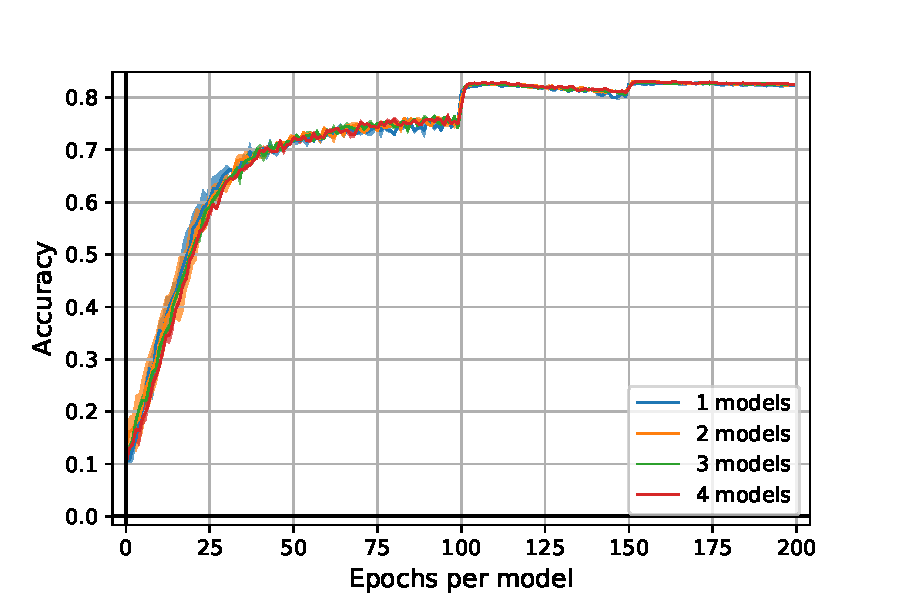
\includegraphics[width=0.49\textwidth]{Images/standard_acc_finalrun_ResNet18_1024_200_0.001.pdf} 
%   \end{minipage}
  
% \caption{On left: Comparison of our algorithm with a standard adversarial training (one model). We reported the results for the model with the best robust accuracy obtained over two independent runs because adversarial training might be unstable. Standard and Robust accuracy ( respectively in the center and on left) on CIFAR-10 test images in function of the number of epochs per classifier with $1$ to $3$ ResNet18 models. The performed attack is PGD with $20$ iterations and $\varepsilon=8/255$.}
% \label{fig:results_cifar}
% \end{center}
% \end{figure*}











% \begin{figure}[!ht]
% 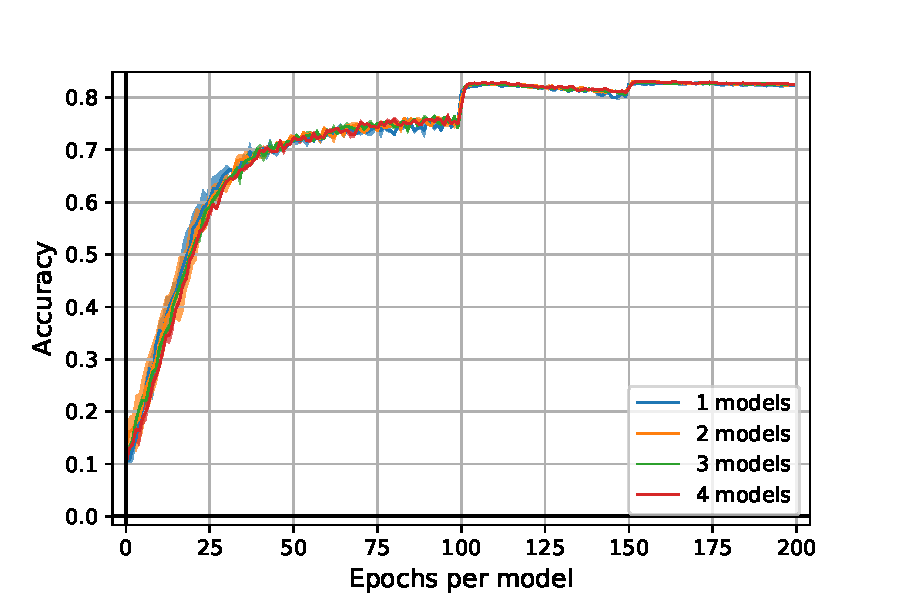
\includegraphics[width=0.46\textwidth]{Images/standard_acc_finalrun_ResNet18_1024_200_0.001.pdf}    \caption{Standard accuracy on CIFAR-10 test images in function of the number of epochs per classifier with $1$ to $3$ ResNet18 models.}
%     \label{fig:plot_standard_acc}
% \end{figure}

% \begin{figure}[!ht]
% 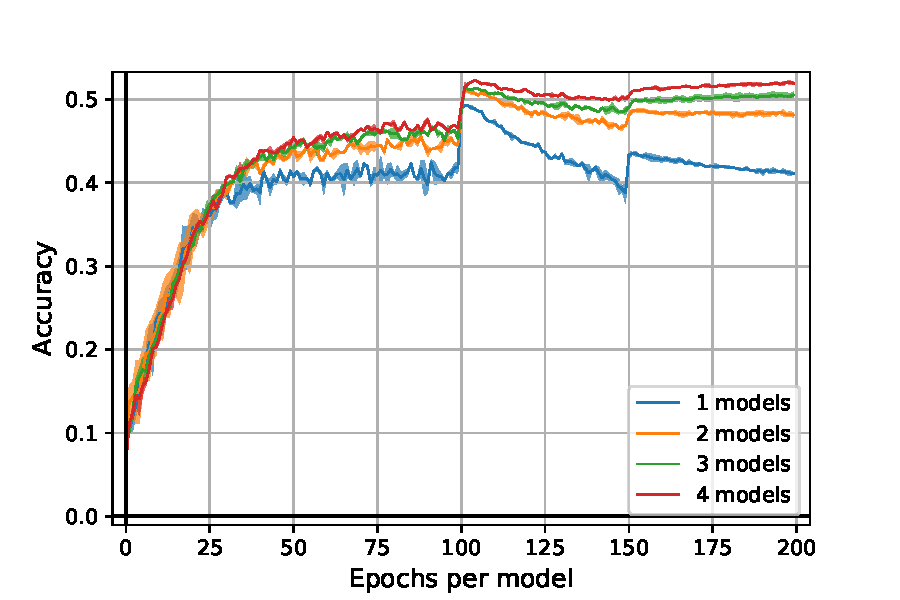
\includegraphics[width=0.46\textwidth]{Images/robust_acc_finalrun_ResNet18_1024_200_0.001.pdf}    \caption{Robust accuracy on CIFAR-10 test images in function of the number of epochs per classifier with $1$ to $3$ ResNet18 models. The attack performed is PGD with $20$ iterations and $\varepsilon=8/255$.}
%     \label{fig:plot_robust_acc}
% \end{figure}



% mettre ca au propre mais les resultats sont la!!

% setup: ResNet18 ou WRN28x10

% Details in supmat: loss +lr + format of training etc

% In supmat: 
% \begin{enumerate}
%     \item details HP (attack + training)
%     \item details runtime
%     \item additional results (with other attacks maybe + other archis...)
    
    
% \end{enumerate}
% Epochs 100
